\documentclass[letterpaper,12pt,fleqn]{article}
\usepackage{matharticle}
\pagestyle{empty}
\newcommand{\ide}{\trianglelefteq}
\begin{document}
\section*{First Ring Isomorphism Theorem}

\begin{theorem}
  Let $\phi:R\to S$ be a homomorphism of rings:
  \[\ker(\phi)\ide R\]
\end{theorem}

\begin{theproof}
  From group theory, we know that $\ker(\phi)$ is an additive subgroup of R \\
  Assume $r\in R$ \\
  Assume $k\in \ker(\phi)$ \\
  $\phi(rk)=\phi(r)\phi(k)=\phi(r)\cdot0=0$ \\
  $rk\in\ker(\phi)$, so $\ker(\phi)$ is a left ideal in $R$ \\
  $\phi(kr)=\phi(k)\phi(r)=0\cdot\phi(r)=0$ \\
  $kr\in\ker(\phi)$, so $\ker(\phi)$ is a right ideal in $R$

  Therefore, by the ideal test, $\ker(\phi)\ide R$.
\end{theproof}

\begin{theorem}
  Let $R$ be a ring and $I\ide R$. $R/I$ is a ring with operations:
  \begin{eqnarray*}
    (a+I)+(b+I) &=& (a+b)+I \\
    (a+I)(b+I) &=& ab+I
  \end{eqnarray*}
\end{theorem}

\begin{theproof}
  From group theory, we already know that $R/I$ is an additive group

  Assume $a,a'\in R$ are representative from the same coset \\
  $a-a'\in I$ \\
  Similarly, assume $b,b'\in R$ are representative from the same coset \\
  $b-b'\in I$

  $(a-a')b=ab-a'b\in I$ \\
  So $ab+I=a'b+I$ \\
  Likewise, $a'(b-b')=a'b-a'b'\in I$ \\
  So $a'b+I=a'b'+I$ \\
  Thus, by transitivity, $ab+I=a'b'+I$

  Now, since all operations are on representative, we inherit all of the properties of
  the operations of $R$, including multiplicative associativity and the distributive
  rules

  Therefore $R/I$ is a ring.
\end{theproof}
\newpage
\begin{theorem}
  Let $R$ be a ring and $I\ide R$, and let $\phi:I\to R/I$ be the canonical homomorphism:
  \[\ker(\phi)=I\]
  Thus, every ideal is the kernel of some homomorphism.
\end{theorem}

\begin{theproof}
  Note that $I$ is the identity for $R/I$

  $x\in\ker(\phi)\iff\phi(x)=I\iff x+I=I\iff x\in I$

  $\therefore\ker(\phi)=I$
\end{theproof}

\begin{theorem}[First (Fundamental) Ring Isomorphism Theorem]
  Let $\phi:R\to S$ be a homomorphism of rings:
  \[R/\ker{\phi}\simeq\phi[R]\]
\end{theorem}

\begin{theproof}
  From group theory, using the canonical injection homomorphism and the first
  (fundamental) group isomorphism theorem, we have:

  \begin{figure}[h]
    \setlength{\leftskip}{1in}
    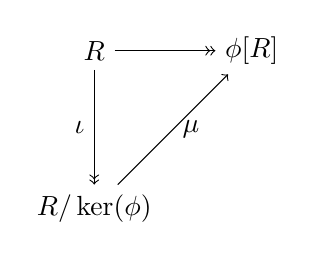
\begin{tikzpicture}
      \node (f) at (0,0) {$R/\ker(\phi)$};
      \node (r) at (0,2) {$R$};
      \node (i) at (2,2) {$\phi[R]$};
      \draw [->>] (r) to (i);
      \draw [->>] (r) to node [left] {$\iota$} (f);
      \draw [->] (f) to node [right] {$\mu$} (i);
    \end{tikzpicture}
  \end{figure}

  So we already know that $\mu:R/\ker{\phi}\to\phi[R]$ is an isomorphism of groups
  where:
  \[r+\ker(\phi)\mapsto\phi(r)\]
  Assume $x,y\in R$
  \begin{eqnarray*}
    \mu((x+\ker(\phi))(y+\ker(\phi))) &=& \mu(xy+\ker(\phi)) \\
    &=& \phi(xy) \\
    &=& \phi(x)\phi(y) \\
    &=& \mu(x+\ker(\phi))\mu(y+\ker(\phi))
  \end{eqnarray*}
  Thus $\mu$ preserves multiplication

  Therefore $\mu$ is a ring isomorphism and $R/\ker{\phi}\simeq\phi[R]$.
\end{theproof}

\end{document}
